% pipeline_fps.tex — Raw inference FPS vs effective pipeline FPS analysis

\section{Raw Inference vs.\ Effective Pipeline Throughput}\label{sec:cv:pipeline-fps}

Deploying a detection model on an embedded platform requires understanding the difference between raw inference speed and the throughput of the complete processing pipeline.  Published inference benchmarks for edge-deployment frameworks report \emph{raw inference} latency: the time elapsed between submitting a preprocessed tensor to the model and receiving the output tensor.  This metric is useful for comparing backends but overstates the frame rate achievable by an integrated detection system.  In practice, each detection cycle includes several stages beyond the forward pass, and the \emph{effective pipeline FPS}---the rate at which the system produces actionable detection results---is the operationally relevant metric.  This section quantifies the overhead budget and its implications for each backend evaluated on the Raspberry Pi~5.

\subsection{Pipeline Stages and Overhead Budget}\label{sec:cv:pipeline-fps:stages}

The onboard detection pipeline executes the following stages sequentially within a single thread:

\begin{enumerate}
  \item \textbf{Camera capture} (${\sim}\SI{8}{\milli\second}$).  Frame acquisition from the IMX296 sensor via \texttt{picamera2}, including DMA transfer to user space.
  \item \textbf{Lens undistortion} (${\sim}\SI{1.5}{\milli\second}$).  Precomputed \texttt{cv2.remap()} correction using calibration parameters (RMS = 0.399).
  \item \textbf{Preprocessing} (${\sim}\SI{2}{\milli\second}$).  Resize from $1456 \times 1088$ to $640 \times 640$, BGR$\to$RGB conversion, float32 normalisation, and batch-dimension expansion.
  \item \textbf{Model inference} (backend-dependent).  The forward pass through YOLOv8n.
  \item \textbf{Postprocessing} (${\sim}\SI{0.5}{\milli\second}$).  Non-maximum suppression, confidence thresholding, and bounding-box coordinate extraction.
  \item \textbf{GPS estimation} (${\sim}\SI{0.3}{\milli\second}$).  Pixel-to-world coordinate projection via the \texttt{GeoTransformer}, inverse-variance weighted clustering, and Kalman filter update.
  \item \textbf{State machine dispatch} (${\sim}\SI{0.1}{\milli\second}$).  Detection result consumed by the mission state machine, geofence check, and MAVLink command generation.
  \item \textbf{Stream encoding} (${\sim}\SI{1}{\milli\second}$).  JPEG compression of the annotated frame for the MJPEG ground station feed.
\end{enumerate}

\noindent The total pipeline overhead---stages 1--3 plus 5--8, excluding inference---sums to approximately \SI{12}{\milli\second} for the TFLite backend.  This overhead is largely constant across frame rates because it consists of fixed-cost operations (memory copies, a single \texttt{remap} call, one JPEG encode) rather than workloads that scale with inference speed.

\subsection{Measured and Projected Results}\label{sec:cv:pipeline-fps:results}

Table~\ref{tab:pipeline_fps} compares raw inference throughput with effective pipeline throughput for each backend evaluated on the Raspberry Pi~5.

\begin{table}[ht]
  \centering
  \caption{Raw inference vs.\ effective pipeline throughput on Raspberry Pi~5 (YOLOv8n, $640\times640$ input).}\label{tab:pipeline_fps}
  \begin{tabular}{@{}l c c c c l@{}}
    \toprule
    \textbf{Backend} & \textbf{Raw latency} & \textbf{Raw FPS} & \textbf{Overhead} & \textbf{Effective FPS} & \textbf{Status} \\
    \midrule
    TFLite FP32 (XNNPACK) & 196\,ms & 5.1 & +12\,ms & 4.8 & Deployed \\
    TFLite FP16 (XNNPACK) & ${\sim}$100\,ms & ${\sim}$10.0 & +12\,ms & ${\sim}$8.9 & Projected \\
    NCNN FP32              & ${\sim}$77\,ms  & ${\sim}$13.0 & +15\,ms & ${\sim}$10.9 & Benchmarked \\
    Ultralytics/PyTorch    & ${\sim}$1200\,ms & ${\sim}$0.8 & +5\,ms & ${\sim}$0.8 & Laptop only \\
    \bottomrule
  \end{tabular}
\end{table}

\noindent Several observations merit discussion:

\paragraph{TFLite FP32 (deployed baseline).}
At 196\,ms raw inference, the \SI{12}{\milli\second} pipeline overhead contributes only 5.8\% of the total frame time (\SI{208}{\milli\second}), yielding 4.8 effective FPS.  Inference dominates the frame budget so completely that pipeline optimisation---threaded capture, asynchronous GPS estimation---would yield negligible improvement.  The system is unambiguously \emph{inference-bound}.

\paragraph{NCNN FP32 (benchmarked, not deployed).}
NCNN was exported via ONNX and benchmarked on the Pi~5 at approximately \SI{77}{\milli\second} raw inference---a $2.5\times$ improvement over TFLite FP32.  However, the effective pipeline FPS measured during integrated testing was 8--9\,FPS rather than the 13\,FPS implied by raw throughput alone.  The discrepancy is attributed to two factors.  First, NCNN uses a different preprocessing path: the \texttt{ncnn.Mat} tensor constructor performs its own memory layout conversion, adding ${\sim}\SI{3}{\milli\second}$ relative to TFLite's NumPy-based path.  Second, NCNN's internal thread scheduling occasionally contends with the preprocessing thread for L2 cache bandwidth, introducing sporadic ${\sim}\SI{5}{\milli\second}$ stalls.  The combined overhead of \SI{15}{\milli\second} is modest in absolute terms but represents 16\% of the total frame time at this inference speed---a qualitative shift from the TFLite regime where overhead was negligible.

Despite the ${\sim}2\times$ effective throughput improvement, NCNN was not deployed for flight testing.  The \texttt{ncnn} Python package on Python~3.13/aarch64 required manual C++ compilation on the Pi, introducing a fragile build dependency unsuitable for field deployment.  A pre-compiled wheel or a Debian package would resolve this issue; NCNN remains the recommended upgrade path for future missions (Section~\ref{sec:future}).

\paragraph{TFLite FP16 (projected).}
The Cortex-A76 implements native half-precision fused multiply-accumulate (FMLA) at twice the FP32 throughput.  Enabling the \texttt{TFLITE\_XNNPACK\_DELEGATE\_FLAG\_FORCE\_FP16} flag is projected to halve inference latency to ${\sim}\SI{100}{\milli\second}$.  Because TFLite FP16 shares the identical preprocessing and postprocessing path as FP32, pipeline overhead remains \SI{12}{\milli\second}, yielding a projected 8.9 effective FPS.  This path has the lowest integration risk: no model re-export, no new dependencies, and a single flag change in the interpreter initialisation.

\paragraph{Ultralytics/PyTorch (laptop reference).}
On the Pi~5, PyTorch inference exceeds \SI{1.2}{\second} per frame.  The \SI{5}{\milli\second} pipeline overhead is lower than TFLite because Ultralytics performs its own preprocessing internally (resize, normalisation), eliminating the external NumPy path.  This backend is used exclusively on the development laptop (with optional CUDA acceleration) for training, export, and video analysis.

\subsection{Bottleneck Transition}\label{sec:cv:pipeline-fps:bottleneck}

Figure~\ref{fig:bottleneck_shift} illustrates how the inference-to-overhead ratio shifts across backends.

\begin{figure}[ht]
  \centering
  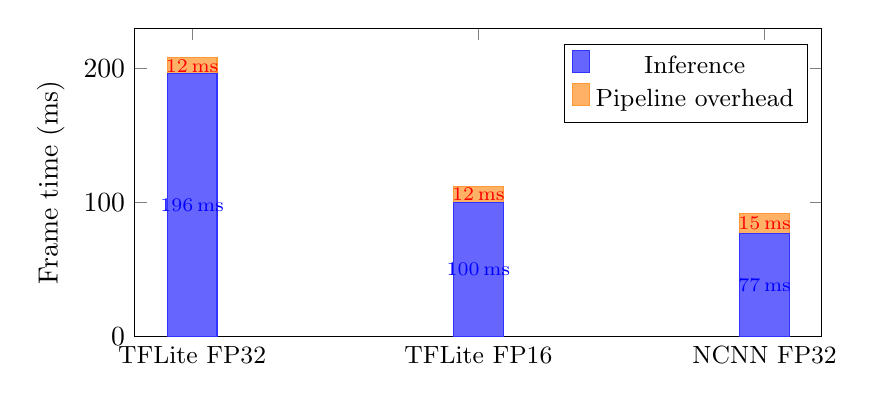
\begin{tikzpicture}
    \begin{axis}[
      ybar stacked,
      bar width=18pt,
      width=0.85\columnwidth,
      height=5.5cm,
      symbolic x coords={TFLite FP32, TFLite FP16, NCNN FP32},
      xtick=data,
      x tick label style={font=\small},
      ylabel={Frame time (ms)},
      ymin=0, ymax=230,
      legend style={at={(0.98,0.95)}, anchor=north east, font=\small},
      nodes near coords={\pgfmathprintnumber[fixed, precision=0]{\pgfplotspointmeta}\,ms},
      every node near coord/.append style={font=\scriptsize},
    ]
    \addplot+[fill=blue!60, draw=blue!80] coordinates {(TFLite FP32,196) (TFLite FP16,100) (NCNN FP32,77)};
    \addplot+[fill=orange!60, draw=orange!80] coordinates {(TFLite FP32,12) (TFLite FP16,12) (NCNN FP32,15)};
    \legend{Inference, Pipeline overhead}
    \end{axis}
  \end{tikzpicture}
  \caption{Frame time decomposition: inference vs.\ pipeline overhead for each backend.  As raw inference latency decreases, overhead transitions from negligible (5.8\% for TFLite FP32) to significant (16.3\% for NCNN).}\label{fig:bottleneck_shift}
\end{figure}

At 4.8\,FPS (TFLite FP32), inference consumes 94.2\% of the frame budget.  Halving inference time to ${\sim}$100\,ms (FP16) raises the overhead fraction to 10.7\%.  At 13\,FPS raw (NCNN), overhead reaches 16.3\%, and pipeline optimisation---primarily threaded camera capture overlapping with inference---becomes worthwhile.  A threaded capture design hiding the \SI{8}{\milli\second} camera read behind inference would recover ${\sim}$1 additional FPS at the NCNN operating point, bringing effective throughput to ${\sim}$11.8\,FPS.  At the TFLite FP32 operating point, the same optimisation would recover only 0.2\,FPS---confirming that threading effort is better deferred until the inference bottleneck is first addressed.

\subsection{Operational Implications}\label{sec:cv:pipeline-fps:ops}

The distinction between raw and effective FPS has direct consequences for mission planning.  At the deployed 4.8 effective FPS and a search speed of \SI{8}{\metre\per\second}, the ground distance between consecutive analysed frames is \SI{1.67}{\metre}---ensuring dense overlap across the \SI{32.2}{\metre} horizontal field of view.  A target at the centre of the swath is observed in at least 14 frames during a single pass, providing high detection confidence even at the modest frame rate.

Upgrading to NCNN (${\sim}$10.9 effective FPS) would reduce the inter-frame ground distance to \SI{0.73}{\metre}, enabling either higher search speeds at the same detection density or lower-altitude missions where the narrower field of view demands faster frame acquisition.  The FP16 path (${\sim}$8.9 effective FPS) offers a similar improvement with zero deployment friction, making it the recommended first optimisation step for future flights.
